\documentclass[12pt,english,nohyper]{tufte-handout}\usepackage[]{graphicx}\usepackage[]{color}
%% maxwidth is the original width if it is less than linewidth
%% otherwise use linewidth (to make sure the graphics do not exceed the margin)
\makeatletter
\def\maxwidth{ %
  \ifdim\Gin@nat@width>\linewidth
    \linewidth
  \else
    \Gin@nat@width
  \fi
}
\makeatother

\definecolor{fgcolor}{rgb}{0.345, 0.345, 0.345}
\newcommand{\hlnum}[1]{\textcolor[rgb]{0.686,0.059,0.569}{#1}}%
\newcommand{\hlstr}[1]{\textcolor[rgb]{0.192,0.494,0.8}{#1}}%
\newcommand{\hlcom}[1]{\textcolor[rgb]{0.678,0.584,0.686}{\textit{#1}}}%
\newcommand{\hlopt}[1]{\textcolor[rgb]{0,0,0}{#1}}%
\newcommand{\hlstd}[1]{\textcolor[rgb]{0.345,0.345,0.345}{#1}}%
\newcommand{\hlkwa}[1]{\textcolor[rgb]{0.161,0.373,0.58}{\textbf{#1}}}%
\newcommand{\hlkwb}[1]{\textcolor[rgb]{0.69,0.353,0.396}{#1}}%
\newcommand{\hlkwc}[1]{\textcolor[rgb]{0.333,0.667,0.333}{#1}}%
\newcommand{\hlkwd}[1]{\textcolor[rgb]{0.737,0.353,0.396}{\textbf{#1}}}%

\usepackage{framed}
\makeatletter
\newenvironment{kframe}{%
 \def\at@end@of@kframe{}%
 \ifinner\ifhmode%
  \def\at@end@of@kframe{\end{minipage}}%
  \begin{minipage}{\columnwidth}%
 \fi\fi%
 \def\FrameCommand##1{\hskip\@totalleftmargin \hskip-\fboxsep
 \colorbox{shadecolor}{##1}\hskip-\fboxsep
     % There is no \\@totalrightmargin, so:
     \hskip-\linewidth \hskip-\@totalleftmargin \hskip\columnwidth}%
 \MakeFramed {\advance\hsize-\width
   \@totalleftmargin\z@ \linewidth\hsize
   \@setminipage}}%
 {\par\unskip\endMakeFramed%
 \at@end@of@kframe}
\makeatother

\definecolor{shadecolor}{rgb}{.97, .97, .97}
\definecolor{messagecolor}{rgb}{0, 0, 0}
\definecolor{warningcolor}{rgb}{1, 0, 1}
\definecolor{errorcolor}{rgb}{1, 0, 0}
\newenvironment{knitrout}{}{} % an empty environment to be redefined in TeX

\usepackage{alltt}
\usepackage[T1]{fontenc}
\usepackage[utf8]{inputenc}
\usepackage{longtable}
\usepackage{wrapfig}
\usepackage{hyperref}
\usepackage{graphicx}
\usepackage[space]{grffile}
\usepackage{geometry}
\usepackage{pgffor}
%\usepackage{caption}
\usepackage{calc}
\usepackage{enumitem}
\usepackage{microtype}
%\usepackage{floatrow} % test for caption below
\usepackage{tabularx}
%\usepackage[capposition=bottom]{floatrow}
\IfFileExists{upquote.sty}{\usepackage{upquote}}{}
\begin{document}



\centerline{\Large\bf Statistics 101 Homework Short Report for Topic 01 LM}
\vspace{1cm}

\begin{marginfigure}
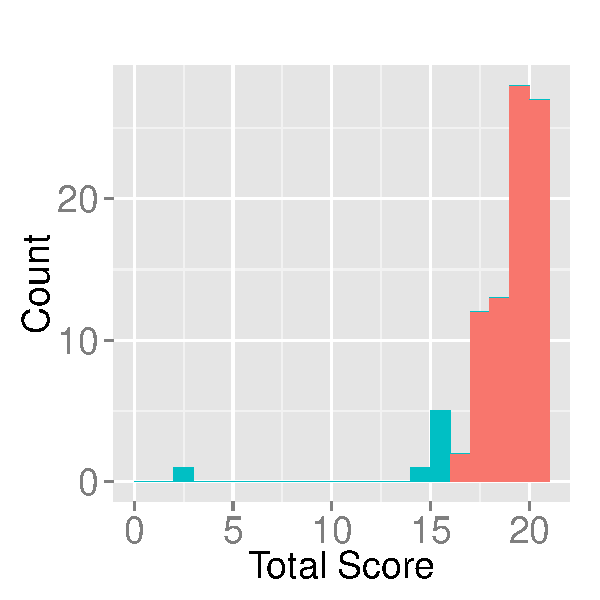
\includegraphics[width=0.98\linewidth]{Topic01_LM_score}
\caption{\label{mar:hist}Histogram of scores. Blue data represent scores less than 80 percent.}
\end{marginfigure}

Each of the 89 students were given 12 questions from a bank of 40 questions. Figure \ref{mar:hist} and Table \ref{tab:summary} give the overall summary of student performance. Table \ref{tab:studentsbelow80} lists the students who did not perform well on this homework. Table \ref{tab:QuestionSet_summary} and Figure \ref{fig:LearningObj_summary} provide summary statistics of the scores per question set and learning outcome.
\bigskip{}

% latex table generated in R 3.1.3 by xtable 1.7-4 package
% Wed Sep  9 17:55:26 2015
\begin{longtable}{llllllll}
  \hline
Mean & Std.dev &   & Min & Q1 & Median & Q3 & Max \\ 
  \hline
18.35 & 2.29 &  & 2.00 & 18.00 & 19.00 & 20.00 & 20.00 \\ 
  (92\%) & (11\%) &  & (10\%) & (90\%) & (95\%) & (100\%) & (100\%) \\ 
   \hline
\hline
\caption{Summary statistics of the scores} 
\label{tab:summary}
\end{longtable}




\begin{fullwidth}
\makeatletter\setlength\hsize{\@tufte@fullwidth}\makeatother
% latex table generated in R 3.1.3 by xtable 1.7-4 package
% Wed Sep  9 17:55:26 2015
\begin{longtable}{rr|lr|lr|lr}
  \hline
  & \% Correct &   & \% Correct &   & \% Correct &   & \% Correct \\ 
  \hline
bskank & 75.00 & maurstad & 75.00 & zacharyt & 75.00 & areuter & 10.00 \\ 
  kehughes & 75.00 & sully81 & 75.00 & colen & 70.00 &  &  \\ 
   \hline
\hline
\caption{Students whose correct percentages are less than 80\%.} 
\label{tab:studentsbelow80}
\end{longtable}

\end{fullwidth}



\vspace{-2mm}

\noindent
\underline{Topic 01 Learning Outcomes:}
\vspace{2mm}

\begin{fullwidth}
\begin{enumerate}[label=\Alph*.,itemsep=-\parsep,leftmargin=*]
  \item
Identify the context of the data by answering the 5 W questions (who, what, where, when, why and how).
\item Identify the who and what questions of data based on the structure of the data table.
\item Determine the structure of the data table based on given information.
\item Determine whether variables are used as quantitative or categorical variables.
\item Identify units for a quantitative variable.
\item Identify categories for a categorical variable.
\item Distinguish between population and sample in a given scenario.

\end{enumerate}
\end{fullwidth}



\vspace{5mm}

%\begin{fullwidth} %ADDED NOW
%\makeatletter\setlength\hsize{\@tufte@fullwidth}\makeatother %ADDED NOW
%\begin{centering}
\begin{figure}[!ht]
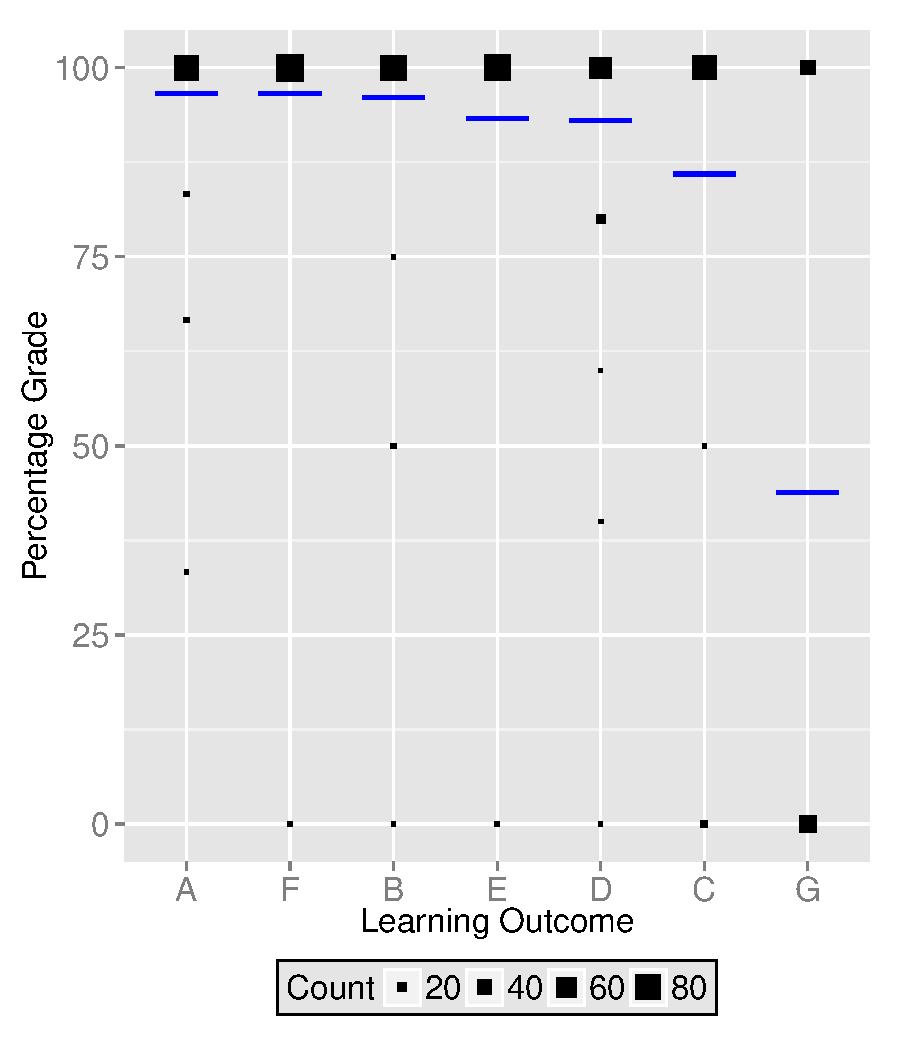
\includegraphics[width=\linewidth]{Topic01_LM_LearningObj_boxplot.pdf}
\caption{Fluctuation diagram of percentage correct by learning outcome. Mean scores are drawn as blue bars.}
\label{fig:LearningObj_summary}
\end{figure}
%\end{centering}
%\end{fullwidth} %ADDED NOW

\begin{fullwidth}
\makeatletter\setlength\hsize{\@tufte@fullwidth}\makeatother
% latex table generated in R 3.1.3 by xtable 1.7-4 package
% Wed Sep  9 17:55:26 2015
\begin{longtable}{cc|ccc|ccc}
  \hline
LO & Qset & \# & Mean & Std.dev & Min & Median & Max \\ 
  \hline
A & A &   4 & 96.63 & 10.71 & 33.33 & 100.00 & 100.00 \\ 
  F & F &   6 & 96.63 & 18.15 & 0.00 & 100.00 & 100.00 \\ 
  B & B &   4 & 96.07 & 15.03 & 0.00 & 100.00 & 100.00 \\ 
  E & E &   8 & 93.26 & 25.22 & 0.00 & 100.00 & 100.00 \\ 
  D & D &  10 & 93.03 & 15.70 & 0.00 & 100.00 & 100.00 \\ 
  C & C &   5 & 85.96 & 34.53 & 0.00 & 100.00 & 100.00 \\ 
  G & G &   3 & \color{red}{43.82} & 49.90 & 0.00 & 0.00 & 100.00 \\ 
   \hline
\hline
\caption{Summary statistics of the question sets. Rows are sorted by mean scores, which are marked red if less than 80 percent.} 
\label{tab:QuestionSet_summary}
\end{longtable}

\end{fullwidth}

\end{document}
